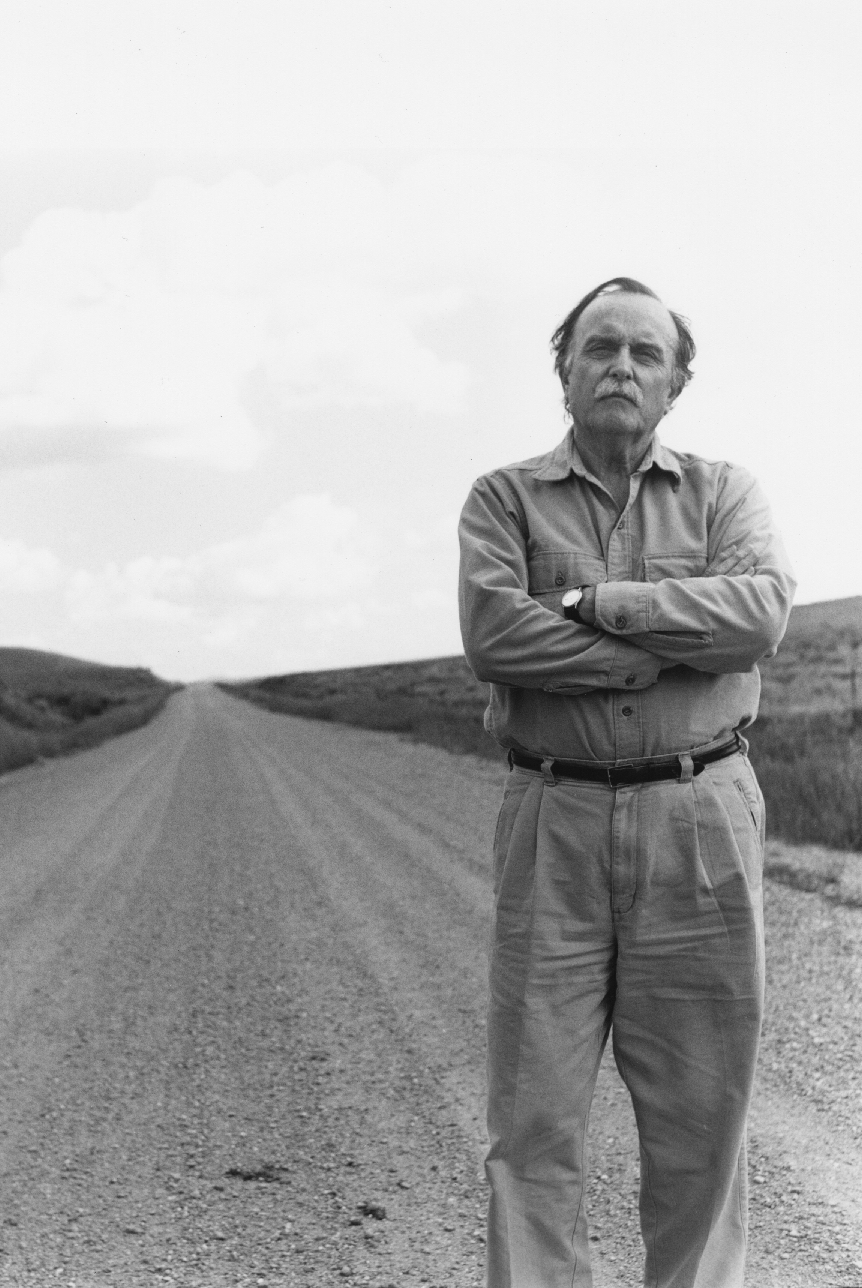
\includepdf[scale=1.1]{lucier/lucier_road_cc.pdf}

%-------------------------------------------------------------
%------------------------------- ALVIN LUCIER - EVER PRESENT -
%-------------------------------------------------------------

\chapter*{Alvin Lucier. \\
			\emph{Waves Song}. 1998\\
			\emph{Ever Present}. 2002}
\addcontentsline{toc}{chapter}{Alvin Lucier. \emph{Waves Song}. 1998 -- Ever Present. 2002}

	\begin{flushright}
		\textit{Nella nostra anima c'� una incrinatura che, se sfiorata, \\
		risuona come un vaso prezioso riemerso dalle profondit� della terra} \\
		Wassilly Kandinsky - \emph{Lo Spirituale nell'Arte}
	\end{flushright}

	\begin{flushright}
		\textit{Music of Changes // John ChAnGEs} \\
		Pierre Boulez
	\end{flushright}

	\begin{flushright}
		\textit{Si dice che i compositori abbiano orecchio per la musica e \\
		di solito significa che non sentono nulla che arrivi alle loro orecchie. \\
		Le loro orecchie sono murate dai suoni di loro creazione.} \\
		John Cage - \emph{45' for a Speaker} (1954)
	\end{flushright}

\bigskip

\begin{multicols}{2}

\begin{quote}
	On 24 September 1960, I attended a concert by John Cage, David Tudor, Merce Cunningham and Carolyn Brown at La
	Fenice Theater in Venice. I had come to Venice that summer on a Fulbright Scholarship to study at the Benedetto
	Marcello Conservatory before going on to Rome where I would spent the next 2 years. The Cage-Tudor event came
	like a bolt out of the blue-all the protocols of the concert situation were violated.
	The concert began, as I remember, with David Tudor striding down the aisle of the theatre and diving under 
	the piano, hitting the underside to make the first sound of the concert. Cage made an appearance playing
	a piano that rose up into the pit hydraulically. The four per- formers had cards upon which were written instructions
	regarding sound s or actions to be made and where to make them. The entire theatre was used-stage, aisles, balconies.
	The work was \emph{Music Walk with Dancers} (1958). During that concert a man walked down the aisle and struck the piano
	with an umbrella and announced: "Now I am composer!" At the height of the pandemonium, Cage was tuning a radio 
	that he used as a sound source, and the Pope came on asking for peace on earth.	
	
	That concert forever altered the way I thought about mu- sic. Until that time I had followed the conventional pattern of
	composer-performer-audience relationships. One would compose a work, wait for some soloist, ensemble or orchestra to perform it, then hope that the audience would like it. It was a lonely life; a waiting game. 
\end{quote}

di John Cage, in luogo degli antichi Greci, come avrebbe continuato Kandinsky.
Ci deve essere un certo grado di consapevolezza in relazione al livello di
comprensione-incomprensione del pensiero di John Cage. Ma ammettendo di
averlo compreso, per quanto noi potremmo approfondire lo studio del suo
pensiero e della sua musica, potremmo solo arrivare ad imitarne alcuni tratti
stilistici. E se tentassimo di


\end{multicols}